\documentclass[border=4pt]{standalone}
\usepackage{amssymb}
\usepackage{tikz}

\begin{document}
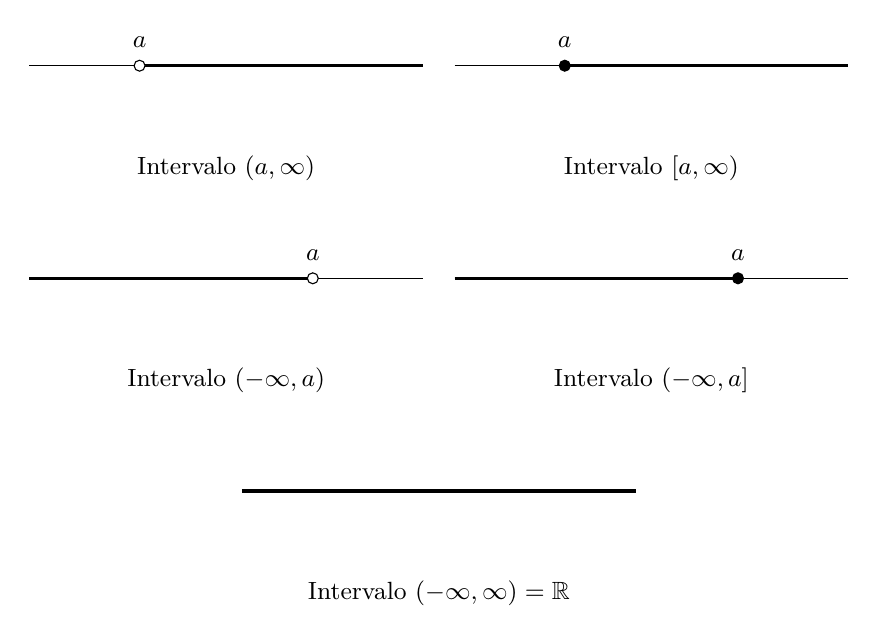
\begin{tikzpicture}[x=1cm, y=1cm, font=\small,
    abierto/.style={circle, draw, fill=white, inner sep=1.4pt},
    cerrado/.style={circle, draw, fill=black, inner sep=1.4pt}]

    % intervalos hacia la derecha: #1 = desplazamiento, #2 = estilo, #3 = etiqueta
    \newcommand{\haciaderecha}[3]{%
        \begin{scope}[shift={#1}]
            \draw (0,0) -- (5,0);
            \draw[very thick] (1.4,0) -- (5,0);
            \node[#2] at (1.4,0) {};
            \node[above=3pt] at (1.4,0) {$a$};
            \node at (2.5,-1.3) {Intervalo #3};
        \end{scope}}
    % intervalos hacia la izquierda
    \newcommand{\haciaizquierda}[3]{%
        \begin{scope}[shift={#1}]
            \draw (0,0) -- (5,0);
            \draw[very thick] (0,0) -- (3.6,0);
            \node[#2] at (3.6,0) {};
            \node[above=3pt] at (3.6,0) {$a$};
            \node at (2.5,-1.3) {Intervalo #3};
        \end{scope}}

    \haciaderecha{(0,0)}{abierto}{$(a,\infty)$}
    \haciaderecha{(5.4,0)}{cerrado}{$[a,\infty)$}
    \haciaizquierda{(0,-2.7)}{abierto}{$(-\infty,a)$}
    \haciaizquierda{(5.4,-2.7)}{cerrado}{$(-\infty,a]$}

    % toda la recta
    \draw[very thick] (2.7,-5.4) -- (7.7,-5.4);
    \node at (5.2,-6.7) {Intervalo $(-\infty,\infty)=\mathbb{R}$};

\end{tikzpicture}
\end{document}
